\chapter{Core modules}

\begin{figure}[b]
	\centering
	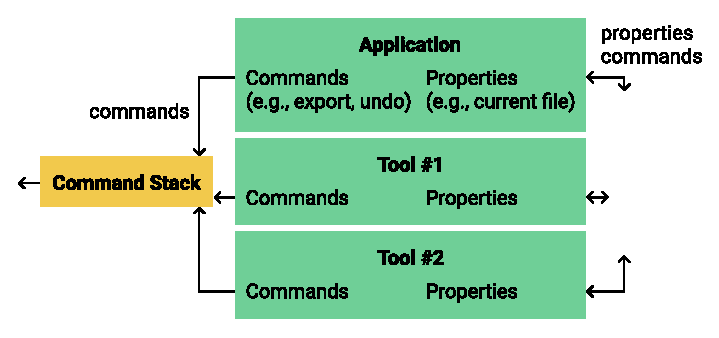
\includegraphics[scale=0.9]{images/architecture_commandstack}
	\caption{The part of architecture covered in this chapter.}
	\label{fig:architecture_commandstack}
\end{figure}

This chapter takes a closer look at the portion of the architecture higlighted in Figure \ref{fig:arch}. We will explain how each task is performed once the UI element has received the input from the user. The UI portion of the architecture will be covered in the next chapter.

% TODO: WARNING: CAREFUL, JE UI NEXT NEBO PREVIOUS CHAPTER?

\section{Commands}
Commands are the primary means of altering the geometry model. Each of them gets executed and placed on the command stack, which allows for the \textit{Undo and Redo} operations to function correctly. The commands then interact with the geometry model (this interaction will be explained in greater detail in the chapter regarding the geometry model) to modify it according to the user's wishes.

Because each command gets put on the command stack, and each Undo step removes one command from the stack, each command has to have a visual impact on the user's work. This means that internal computations, such as geometry queries, cannot be represented as commands, because pressing the Undo button would not have any visual effect and would confuse the user. Examples of commands include: coloring a single triangle (triangle painter tool), adding a brush stroke (as in semi-automatic segmentation we looked at in Chapter 2) or a single step of triangle mesh subdivision.

\subsection*{Implementation details}

A command will be a class with three primary methods.
\begin{itemize}
\item \textit{constructor} -- Once the command gets created, the main thing to do is remember the state the geometry model was in before the command modified it. This will allow for the command to restore the model if \textit{Undo} is pressed. The advantage of saving the state in the constructor and not in the execute function itself is because of the \textit{Redo} mechanism -- if the user repeatedly presses the combination of \textit{Undo + Redo}, the model gets saved only once as opposed to each execute.
\item \textit{execute()} -- The execute function will perform the task the command is created to do. This will typically get called immediately before the command gets placed onto the command stack.
\item \textit{undo()} -- This method will take the state of the model saved by the constructor of the command and apply it to the current geometry model, effectively reversing the command.
\end{itemize}

\section{Command Manager and Command Stack}

\subsection{Command Stack}

As the name suggests, the Command Stack is a \textit{LIFO} type structure, its main purpose to store the executed commands to allow for the \textit{Undo and Redo} operations to be performed. As we have outlined in the previous section, each command carries all neccessary information to perform both actions. This means that the Command Stack can be a simple container without any significant logic behind it.

\subsection{Command Manager}

The command manager is a object to manage the command stack. It receives the commands from tools, executes them and stores them in the command stack. When the user wishes to \textit{Undo} an operation, the command manager retrieves the top command from the stack and invokes its undo() method.

\section{Tools}

A tool is the main programable component which connects the low-level command structure we outlined above and the high-level UI components (such as color-pickers, the user performing brush strokes and file operations like exporting the file). This design should also allow for later advancements of the software easily -- adding a tool to the software should be a matter of writing the new tool's Tool class, unless the tool is advanced and needs some complicated custom geometry processing functions.

Each tool is composed of two main components:
\begin{itemize}
\item \textit{properties} -- a methodless object holding the tool's properties which can be customized by the user. This includes, for example, the color which gets assigned to the triangles in the triangle painter tool, the number of colors for automatic-segmentation, the subdivision level or the gradient thresholds for region detection in bucket painting. The information in this object gets changed directly when the user interacts with the UI.

\item \textit{commands} -- Each tool generates at least one command, which it creates, fills with all neccessary information the command needs to execute itself, and passes it to the command manager. More complicated tools can create more commands, as we will illustrate in the following section. The tool is able to do some pre-processing before a command is issued, in case the pre-processing isn't visible on the screen, as shown in example 4.1.

\end{itemize}

\section{Examples of data flow within the center section of the achitecture}

We include a few example use cases which should illustrate what happens in the application (normal font) when a user interacts with the UI (italics). The first example shows the need for preprocessing power within the tool class, while the second example illustrates the need for multi-command tools.

\subsection{A preprocessing example - triangle painter}
\textit{The user selects the triangle painter from the tool box, and in the Side Pane, he changes the color from default red to green.}

This action makes the UI manager change the color property of the TrianglePainter tool from red to green.

\textit{The user then clicks on a triangle that he sees on the screen, in Model View.}

This makes the UI generate a ray in a direction of the user's mouse input. It then calls the TrianglePainter tool, passes the ray and tells it to color it, according to the tool's settings. The tool first calls the Geometry Model, to retrieve the triangle that gets intersected by the given ray, then creates a command to color the triangle with the color it has in its properties. The command is then passed to the CommandManager and executed. The query for the ray intersection is not passed as a command, because it is not visible for the user, hence should not be reversible.

\subsection{A multicommand tool example - the semi-automatic segmentation tool}
\textit{The user selects the number of colors -- 4. The user also selects which colors he would like to use -- C, M, Y, K.}

The UI updates the tool's properties to reflect these values.

\textit{The user then selects the color C, and performs a stroke.}

The UI first tells the tool that the current color is C. Then the tool receives the parameters of the stroke (much like the ray for a click), creates the command for a stroke with color C and sends it to the command manager.

This gets repeated for the other 3 colors. So far the tool generated 4 commands. If at any point the user presses Ctrl + Z, only one of the strokes disappears.

\textit{The user confirms the hint strokes are complete and the segmentation can start.}

The tool now generates the final command to complete the segmentation and passes it to the manager.


If the user presses Ctrl + Z now, only the segmentation will get removed, with the strokes still remaining on the object.

\section{Geometry model}

The geometry model is responsible for keeping the geometry data (triangles of the model) in memory and implementing geometric operations, that then get used in commands, to perform the tasks specified by the tools.

\subsection{Implementation variants}

There are two main approaches to programming the geometry model. One approach is to look at the model as a state-less chunk of data. The functions that operate on the model (e.g. \textit{return the triangle that intersects this ray}) are free functions that just get called on the geometry model. The second approach is to implement the model as a full object. This means that the model has its private data -- the triangles of the user's model, and it has its methods -- the geometric operations it allows the user (i.e. the programmer of the commands and tools) to perform upon the private data.

Both solutions have their pros and cons and we, at the time of writing, do not know which will shape up to be a better fit to the application. We will briefly mention some of the reasons we might choose either one. The state-less \textit{struct} version is better for handling the data. We will need to make some kinds of copies both for saving the model on the disc and for the \textit{undo Undo and Redo} operations. This approach would allow us to simply copy the struct and not waste any space or time. The object-oriented approach is easier to work with and probably less confusing for new programmers trying to implement a new tool or other extensions to the application.

\subsection{Libraries}

There are several libraries that the geometry model could benefit from. We have been searching on the internet and did research and we found the following libraries that we will try to use to augment the geometry model.

\begin{itemize}
\item \textbf{Assimp\footnote{http://www.assimp.org/}} -- a portable Open Source library to import various well-known 3D model formats in a uniform manner\footnote{Description taken from http://www.assimp.org/}. This library is very important to our application as it will allow us to support a plethora of 3D formats for the users to use. This should help the less experienced users by not forcing them to convert their objects to different formats before our program can import them.

\item \textbf{cereal\footnote{https://uscilab.github.io/cereal/}} -- cereal is a header-only C++11 serialization library. cereal takes arbitrary data types and reversibly turns them into different representations, such as compact binary encodings\footnote{Description taken from https://uscilab.github.io/cereal/}. We need to serialize data to enable saving the current state of the user's project on disc, and then be able to de-serialize them when the user wishes to continue working on the saved project and presses \textit{load existing project}. We have had positive experience with cereal and that is the reason we chose this library.

\item \textbf{The Computational Geometry Algorithms Library or CGAL\footnote{https://www.cgal.org/}} -- a software project that provides easy access to efficient and reliable geometric algorithms in the form of a C++ library\footnote{Description taken from https://www.cgal.org/}. We have heard very positive feedback on CGAL and therefore will attempt to use the library for the more complex geometry problems. We have, however, not had any previous experiences with CGAL, so we are unsure as to how well it will fulfill our requirements and might drop the use of it if it does not meet our expectations.
\end{itemize}